\subsection{Ola Compiler Backend: from LLVM IR to OlaVM assembly}

Ola compiler backend bridge IR structure of module, function and Instruction Set Architecture(ISA) related callconv, registers and instructions.
Its main features are code generation related lower and optimization related passes.

Target ISA mainly contains custom target instructions, registers which contain register class and register information, call convention and datalayout information.

Module in addition to inheritance IR is parsed out as Module structure, the description of its function and differ significantly with LLVM IR.
Data information of Basic Block(BB) in the instructions target for the instruction, the register contains VRegs(Virtual Registers) and RegUnit(Register Unit) two categories, and contains a VRegs to Instructions(Insts) mapping.
At the same time, instruction in data layout is referred to target instruction. Note that the structure of slot which contains stack base pointer and stack offset describe the memory access operations of parameters, local variables.

The lower provides the process of downgrading IR instruction to target instruction. Specifically it also requires copy parameters to VRegs for function call.

The pass module contains the register allocation(RegAlloc, RA) and spiller for analyzing the liveness of the pass and the function pass.

\subsubsection{Backend introduction}

The backend of the Ola compiler compiles ir into target assembly code. It takes the llvm std ir generated by the frontend as input and the ola assembly code as output.

Its pipeline process is as follows:
\begin{figure}[!htbp]
    \centering
    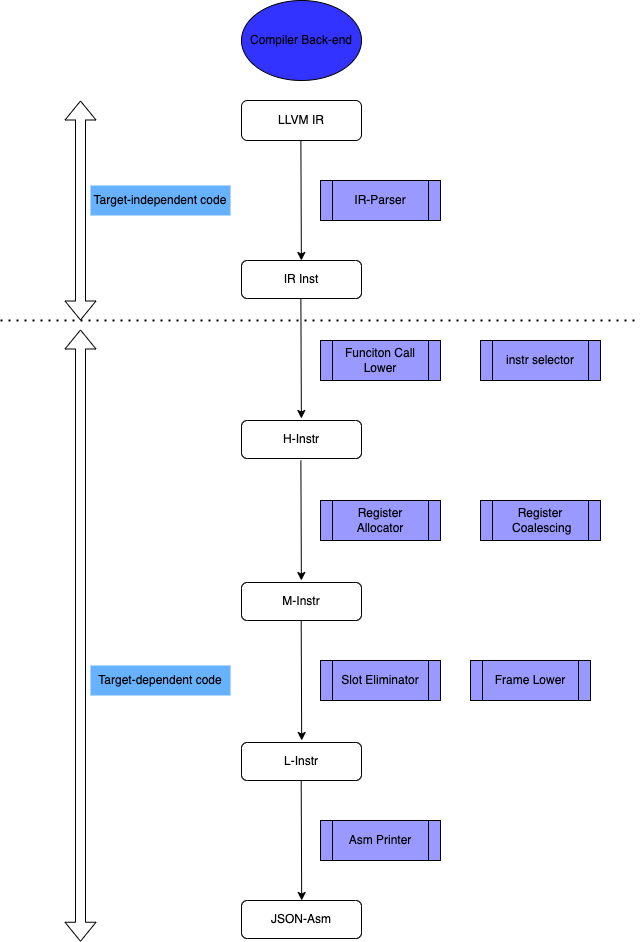
\includegraphics[width=0.6\textwidth]{ola-lang-backend.jpg}
    \caption{ola-lang backend pipeline}
    \label{fig:ola-lang-backend}
\end{figure}

An example ola-lang ola assembly code for computing sqrt of type u32 with prophet version is as follows:
\begin{lstlisting}[language={}]
{
  "program": "u32_sqrt:\n.LBL3_0:\n  mov r3 r1\n  mov r1 r3\n.PROPHET3_0:\n  mov r0 psp\n  mload r0 [r0,0]\n  range r0\n  mul r2 r0 r0\n  assert r2 r3\n  ret\nmain:\n.LBL4_0:\n  add r8 r8 4\n  mstore [r8,-2] r8\n  mov r1 4\n  call sqrt_test\n  add r8 r8 -4\n  end\nsqrt_test:\n.LBL5_0:\n  add r8 r8 6\n  mstore [r8,-2] r8\n  mov r0 r1\n  mstore [r8,-3] r0\n  mload r1 [r8,-3]\n  call u32_sqrt\n  mstore [r8,-4] r0\n  mload r0 [r8,-4]\n  add r8 r8 -6\n  ret\n",
  "prophets": [
    {
      "label": ".PROPHET3_0",
      "code": "%{\n    entry() {\n        cid.y = sqrt(cid.x);\n    }\n%}",
      "inputs": [
        "cid.x"
      ],
      "outputs": [
        "cid.y"
      ]
    }
  ]
}
\end{lstlisting}

An example ola-lang ola assembly code for computing sqrt of type u32 with instructions version is as follows:
\begin{lstlisting}[language={}]
{
  "program": "main:\n.LBL5_0:\n  add r8 r8 4\n  mstore [r8,-2] r8\n  mov r1 4\n  call sqrt_test\n  add r8 r8 -4\n  end\nsqrt_test:\n.LBL6_0:\n  add r8 r8 19\n  mstore [r8,-16] r1\n  mov r1 0\n  mstore [r8,-17] r1\n  mload r1 [r8,-16]\n  gte r2 r1 3\n  neq r0 r1 3\n  and r2 r2 r0\n  cjmp r2 .LBL6_1\n  jmp .LBL6_2\n.LBL6_1:\n  mload r0 [r8,-16]\n  mstore [r8,-17] r0\n  mload r0 [r8,-16]\n  mstore [r8,-12] r0\n  mload r0 [r8,-12]\n  mov r1 r0\n  mov r2 2\n.PROPHET6_0:\n  mov r0 psp\n  mload r0 [r0,0]\n  mstore [r8,-11] r0\n  mload r0 [r8,-11]\n  range r0\n  mov r0 2\n  mload r1 [r8,-11]\n  add r4 r1 1\n  not r7 r4\n  add r7 r7 1\n  add r5 r0 r7\n  range r5\n  mload r0 [r8,-12]\n  mov r1 r0\n  mov r2 2\n.PROPHET6_1:\n  mov r0 psp\n  mload r0 [r0,0]\n  range r0\n  mul r1 r0 2\n  mstore [r8,-15] r1\n  mload r1 [r8,-15]\n  mload r2 [r8,-11]\n  add r1 r1 r2\n  mstore [r8,-14] r1\n  mload r1 [r8,-14]\n  mload r2 [r8,-12]\n  assert r1 r2\n  add r0 r0 1\n  mstore [r8,-13] r0\n  mload r0 [r8,-13]\n  range r0\n  mload r0 [r8,-13]\n  mstore [r8,-18] r0\n  mov r0 0\n  mstore [r8,-19] r0\n  jmp .LBL6_4\n.LBL6_2:\n  mload r0 [r8,-16]\n  neq r0 r0 0\n  cjmp r0 .LBL6_10\n  jmp .LBL6_11\n.LBL6_3:\n  mload r0 [r8,-17]\n  add r8 r8 -19\n  ret\n.LBL6_4:\n  mload r0 [r8,-19]\n  mov r1 100\n  gte r1 r1 r0\n  neq r3 r0 100\n  and r1 r1 r3\n  cjmp r1 .LBL6_5\n  jmp .LBL6_7\n.LBL6_5:\n  mload r0 [r8,-18]\n  mload r1 [r8,-17]\n  gte r0 r0 r1\n  cjmp r0 .LBL6_8\n  jmp .LBL6_9\n.LBL6_6:\n  mload r1 [r8,-19]\n  add r0 r1 1\n  mstore [r8,-19] r0\n  jmp .LBL6_4\n.LBL6_7:\n  jmp .LBL6_3\n.LBL6_8:\n  jmp .LBL6_7\n.LBL6_9:\n  mload r0 [r8,-18]\n  mstore [r8,-17] r0\n  mload r0 [r8,-16]\n  mstore [r8,-3] r0\n  mload r0 [r8,-18]\n  mstore [r8,-2] r0\n  mload r0 [r8,-3]\n  mov r1 r0\n  mload r0 [r8,-2]\n  mov r2 r0\n.PROPHET6_2:\n  mov r0 psp\n  mload r0 [r0,0]\n  mstore [r8,-1] r0\n  mload r0 [r8,-1]\n  range r0\n  mload r0 [r8,-1]\n  add r4 r0 1\n  not r7 r4\n  add r7 r7 1\n  mload r0 [r8,-2]\n  add r5 r0 r7\n  range r5\n  mload r0 [r8,-3]\n  mov r1 r0\n  mload r0 [r8,-2]\n  mov r2 r0\n.PROPHET6_3:\n  mov r0 psp\n  mload r0 [r0,0]\n  range r0\n  mload r1 [r8,-2]\n  mul r1 r0 r1\n  mstore [r8,-10] r1\n  mload r1 [r8,-10]\n  mload r2 [r8,-1]\n  add r1 r1 r2\n  mstore [r8,-9] r1\n  mload r1 [r8,-9]\n  mload r2 [r8,-3]\n  assert r1 r2\n  mload r1 [r8,-18]\n  add r0 r0 r1\n  mstore [r8,-5] r0\n  mload r0 [r8,-5]\n  range r0\n  mload r0 [r8,-5]\n  mov r1 r0\n  mov r2 2\n.PROPHET6_4:\n  mov r0 psp\n  mload r0 [r0,0]\n  mov r4 r0\n  range r4\n  mov r0 2\n  add r1 r4 1\n  mstore [r8,-8] r1\n  mload r1 [r8,-8]\n  not r7 r1\n  add r7 r7 1\n  add r0 r0 r7\n  mstore [r8,-7] r0\n  mload r0 [r8,-7]\n  range r0\n  mload r0 [r8,-5]\n  mov r1 r0\n  mov r2 2\n.PROPHET6_5:\n  mov r0 psp\n  mload r0 [r0,0]\n  range r0\n  mul r1 r0 2\n  mstore [r8,-6] r1\n  mload r1 [r8,-6]\n  add r1 r1 r4\n  mstore [r8,-4] r1\n  mload r1 [r8,-5]\n  mload r2 [r8,-4]\n  assert r2 r1\n  mstore [r8,-18] r0\n  jmp .LBL6_6\n.LBL6_10:\n  mov r0 1\n  mstore [r8,-17] r0\n  jmp .LBL6_11\n.LBL6_11:\n  jmp .LBL6_3\n",
  "prophets": [
    {
      "label": ".PROPHET6_0",
      "code": "%{\n    function mod(felt x, felt y) -> felt {\n        return x % y;\n    }\n    entry() {\n        cid.r = mod(cid.x, cid.y);\n    }\n%}",
      "inputs": [
        "cid.x",
        "cid.y"
      ],
      "outputs": [
        "cid.r"
      ]
    },
    {
      "label": ".PROPHET6_1",
      "code": "%{\n    function div(felt x, felt y) -> felt {\n        return x / y;\n    }\n    entry() {\n        cid.q = div(cid.x, cid.y);\n    }\n%}",
      "inputs": [
        "cid.x",
        "cid.y"
      ],
      "outputs": [
        "cid.q"
      ]
    },
    {
      "label": ".PROPHET6_2",
      "code": "%{\n    function mod(felt x, felt y) -> felt {\n        return x % y;\n    }\n    entry() {\n        cid.r = mod(cid.x, cid.y);\n    }\n%}",
      "inputs": [
        "cid.x",
        "cid.y"
      ],
      "outputs": [
        "cid.r"
      ]
    },
    {
      "label": ".PROPHET6_3",
      "code": "%{\n    function div(felt x, felt y) -> felt {\n        return x / y;\n    }\n    entry() {\n        cid.q = div(cid.x, cid.y);\n    }\n%}",
      "inputs": [
        "cid.x",
        "cid.y"
      ],
      "outputs": [
        "cid.q"
      ]
    },
    {
      "label": ".PROPHET6_4",
      "code": "%{\n    function mod(felt x, felt y) -> felt {\n        return x % y;\n    }\n    entry() {\n        cid.r = mod(cid.x, cid.y);\n    }\n%}",
      "inputs": [
        "cid.x",
        "cid.y"
      ],
      "outputs": [
        "cid.r"
      ]
    },
    {
      "label": ".PROPHET6_5",
      "code": "%{\n    function div(felt x, felt y) -> felt {\n        return x / y;\n    }\n    entry() {\n        cid.q = div(cid.x, cid.y);\n    }\n%}",
      "inputs": [
        "cid.x",
        "cid.y"
      ],
      "outputs": [
        "cid.q"
      ]
    }
  ]
}
\end{lstlisting}

The backend data structure contains mainly lists,insts, and mcinsts. The ABI then contains Function call specification and Mapping Relationships to Virtual Memory.

The backend codegen pipeline process:
\begin{itemize}
    \item IR parsing

    \item Function call lowering

    \item Instruction selection

    \item Register Allocation

    \item Slot elimination

    \item Stack frame handling

    \item Assembly printing
\end{itemize}

\subsubsection{Parser: parse LLVM IR to Module insts}

The detailed process is as follows:
    \begin{itemize}
        \item IR parsing

IR is composed of the following structure: module -> function -> value -> types.

(1) Module structure contains Target (triple and datalayout information), Function, Attribute, GlobalVariable.

(2) Function structure contains name, type information, Visibility, Attribute and Parameter list basic information, and data, Layout.

(3) Among them, layout contains the sequential logical relationship between basicBlocks and the instructions within them.

(4) Data contains the specific Value, Instruction, BasicBlock list instances.

(5) BasicBlock is identified by BasicBlockId and consists of two parts: name and number. Each BB block usually contains one preds and one sucs.

(6) Instruction is identified by BasicBlockId+InstructionId and usually consists of Opcode, Operand, dest and the Type of its operation.

(7) Value contains Instruction, Argument, Constant and InlineAsm types.

(8) Due to the characteristics of the instruction set of olavm, the type is currently mainly i64 type.

        \item IR parsing process

process: targetDatalayout/targetTriple -> attributeGroup -> localType -> globalVariable -> function -> metadata.

The function is mainly divided into two parts: parseArgumentList and parseBody.

Its pipeline process is as follow:
\begin{figure}[!htbp]
    \centering
    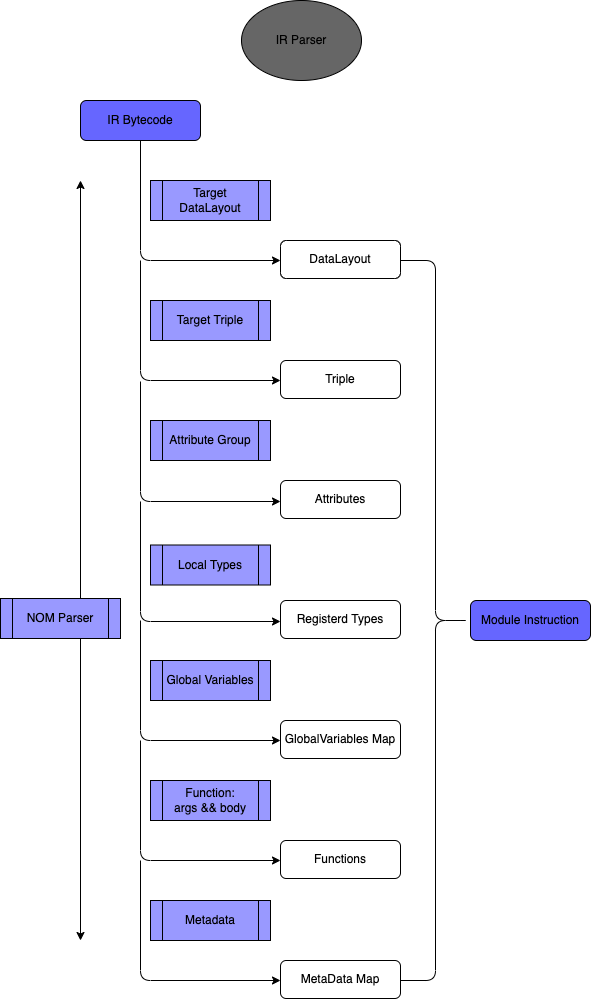
\includegraphics[width=0.6\textwidth]{ola-lang-backend-parser.jpg}
    \caption{ola-lang backend parser pipeline}
    \label{fig:ola-lang-backend-parser}
\end{figure}
\end{itemize}
\subsubsection{Opt: opt pass on IR insts}

Currently DominatorTree is an mainly analysis pass, conversion transform passes contains dce, mem2reg, sccp.

Its pipeline process is as follows:
\begin{figure}[!htbp]
    \centering
    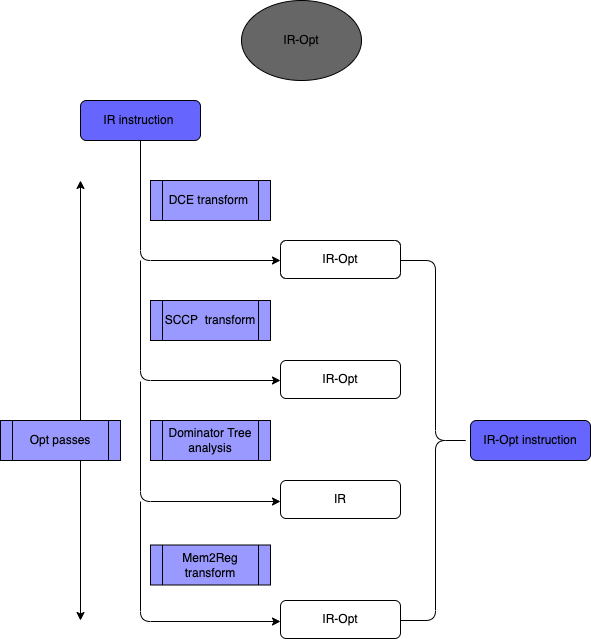
\includegraphics[width=0.5\textwidth]{ola-lang-backend-ir-opt.jpg}
    \caption{ola-lang backend ir opt}
    \label{fig:ola-lang-backend-ir-opt}
\end{figure}
\subsubsection{ISA description: register and insts}

\begin{itemize}
    \item back-end codegen modules

bridging ir structure of module, function, and isa related callconv, register and isa, code generation related lower, and optimization-related pass.

TargetISA main contains custom TargetInst, Register(RegisterClass/RegisterInfo), lower and modulepasses, callconv, datalayout information.

Module in addition to inheritance Ir parsed out Module, the description of its Function and ir differ significantly.

Data information: BasicBlock in the instructions for Target Instruction, the register contains VRegs and RegUnit two categories, and contains a vregtoinsts mapping.
At the same time, Inst in Layout is referred to TargetInst. Note that the memory access operations of parameters, local variables, etc. are described by the structure of slot(ptr+offset).

The lower module provides the process of downgrading LoweringContext to Instruction, and for function calls it also requires copyargstovregs.

The pass module contains the regalloc and spiller for analyzing the liveness of the pass and the function pass.

        \item back-end process

(1) Register and insts description

The register description is as below:
\begin{table}[!ht]
    \resizebox{\textwidth}{!}{
        \begin{tabular}{|c|c|c|}
            \hline
            \textit{Type}  & \textit{Description} & \textit{Register Group}  \\ \hline
            general registers & general used by program &  $[r0-r8] $ \\ \hline
            return regsiter & return value for return to caller &  $[r0] $ \\ \hline
            parameters rigsters & parameters value for passing arguments &  $ [r1, r2, r3] $ \\ \hline
            tmp registers & tmp alloc for local variables &  $[r4, r5, r6, r7]$ \\ \hline
            stack pointer & function's stack pointer &  $[r8] $ \\ \hline
            special registers & interact with vm: pc for program counter and psp for prophet pointer &   $[pc, psp] $ \\ \hline
        \end{tabular}}
    \caption{Register Description}
    \label{table:register-description}
\end{table}

Insts description is as bellow:

Opcode with register or immediate number:
\begin{lstlisting}[language={}]
    ADDri,
    ADDrr,
    MULri,
    MULrr,

    EQri,
    EQrr,
    ASSERTri,
    ASSERTrr,

    MOVri,
    MOVrr,

    JMPi,
    JMPr,
    CJMPi,
    CJMPr,
    CALL,
    RET,
    END,

    MLOADi,
    MLOADr,
    MSTOREi,
    MSTOREr,

    RANGECHECK,
    AND,
    OR,
    XOR,
    NOT,
    NEQ,
    GTE,

    PROPHET,

    Phi,
\end{lstlisting}

Operand data type:
\begin{lstlisting}[language={}]
    Reg(Reg),
    VReg(VReg),
    Int8(i8),
    Int32(i32),
    Int64(i64),
    MemStart,
    Slot(SlotId),
    Block(BasicBlockId),
    Label(String),
    GlobalAddress(String),
    None,
\end{lstlisting}

\end{itemize}
\subsubsection{ABI Lower: Lowering Function Call}
    
Ola Procedure Call Standard(OPCS) are as follows:

The stack initialization points to the first address of the frame stack after the \texttt{fp} register is loaded.
    
The address will be increased when the \texttt{call} instruction is executed later.
When the \texttt{ret} instruction is executed, the \texttt{fp} register points to the address and falls back.
    
    
the Calling process is as follows:
\begin{itemize}
    \item call label

Caller use \texttt{call} instruction to call a callee as \texttt{call functionLabel}, and \texttt{fp} points to the new frame.\par
The \texttt{pc} address returned by the callee is placed in \texttt{fp-1} which is detected by VM but not visible by the compiler backend.\par
Its instructions pattern are as follows:
\begin{lstlisting}[language={}]
main:
.LBL0_0:
  ...
  call foo
  ...
foo:
.LBL1_0:
  ...
\end{lstlisting}
    \item function address

The address pointed to by \texttt{fp} before the function call is placed in \texttt{fp-2} as \texttt{mstore [r8,-2] r8}.\par
Its instructions pattern are as follows:
\begin{lstlisting}[language={}]
mstore [r8,-2] r8
\end{lstlisting}
    \item passing arguments

Function parameter processing: the first three input parameters are placed in the three registers \texttt{r1}, \texttt{r2}, and \texttt{r3}.
If there are more than 3 parameters, start with the fourth input parameter and descend accordingly in \texttt{fp-3}, \texttt{fp-4}, \texttt{...}. \par
Its instructions pattern are as follows:
\begin{lstlisting}[language={}]
mov r1 vreg1
mload r2 [r8,offset]
mov r3 vreg2
\end{lstlisting}
    \item  local variables

Local variables inside the function start at old \texttt{fp}, and their addresses are stored incrementally.

The single return value is stored in \texttt{r0}. If there are multi return values, it needs to be returned by a memory pointer that return the package data.\par
Instruction pattern for single return value is as follows:
\begin{lstlisting}[language={}]
mov r0 vreg3
\end{lstlisting}
\end{itemize}

The call stack frames layout is as follows \ref{fig:ola-lang-backend-functioncall}:

\begin{figure}[!htp]
    \centering
    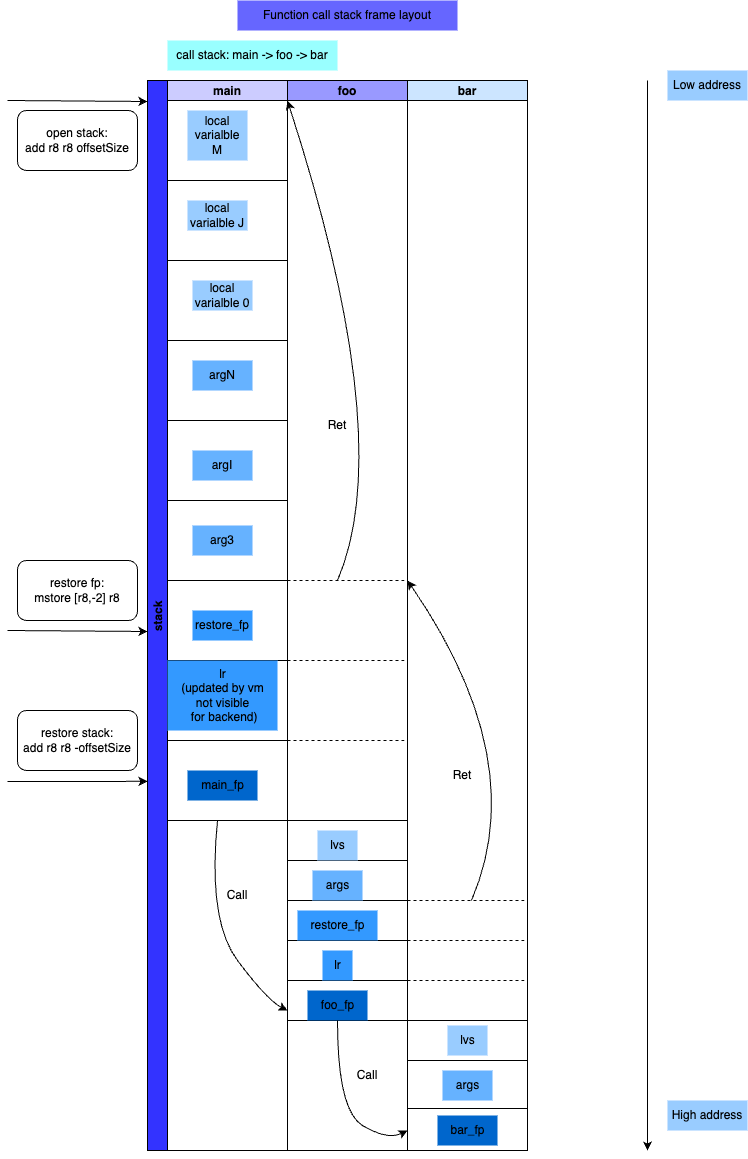
\includegraphics[width=0.8\textwidth]{ola-lang-backend-functioncall.jpg}
    \caption{Ola-lang Function Call Stack Frames}
    \label{fig:ola-lang-backend-functioncall}
\end{figure}

For prophet library functions, its instructions pattern as:
\begin{lstlisting}[language={}]
.PROPHET{funcNum}_{prophetNum}:  // bind to prophet label
mov r0 psp  // interact with prophet read-only memory, get return value from prophet pointer
mload r0 [r0,0]  // used returned r0 as indexed addressing
\end{lstlisting}

First \texttt{.PROPHET} label binds to the prophet instance in assembly output.
Then the program interacts with prophet read-only memory, get the return value from prophet pointer \texttt{[psp]} and write the result into \texttt{r0}.
At last, we use \texttt{r0} as indexed addressing to load return values from prophet memory.
\subsubsection{Insts selection: match pattern from ir inst to MCinst}

It match ir insts opcode + operand pattern, then lower the matched pattern to target machine code insts.

Several common patterns such as: 
\begin{table}[!ht]
    \resizebox{\textwidth}{!}{
        \begin{tabular}{|c|c|}
            \hline
            \textit{Pattern Type} & \textit{Description} \\ \hline
            Alloca  & params and vars allocation \\ \hline
            IntBinary & bianary operator \\ \hline
            Load & memory load \\ \hline
            Store & memory store  \\ \hline
            Call & function call \\ \hline
            Return & function call return \\ \hline
            Branch & branch control flow \\ \hline
            Conditional Branch & conditional branch control flow \\ \hline
        \end{tabular}}
    \caption{Instruction Pattern}
    \label{table:Instruction-pattern}
\end{table}

Let's take Conditional Branch for example, it's target insts as follow:
\begin{table}[!ht]
    \resizebox{\textwidth}{!}{
        \begin{tabular}{|c|c|c|c|}
            \hline
            \textit{operator}  & \textit{Reg+Imm} & \textit{Reg+Reg} & \textit{Cycles}  \\ \hline
            == & \makecell{mov tmpReg imm \\ eq tmpReg regA tmpReg \\ cjmp tmpReg labelTrue} & \makecell{eq tmpReg regA regB \\ cjmp tmpReg labelTrue} & \makecell{3inst + 2reg \\ 2inst + 3reg} \\ \hline
            < & \makecell{mov tmpReg1 imm \\ gte tmpReg1 tmpReg1 regA \\ neq tmpReg2 tmpReg1 regA \\and tmpReg2 tmpReg2 tmpReg1 \\ cjmp tmpReg2 labelTrue} & \makecell{gte tmpReg1 regB regA \\ neq tmpReg2 regA regB \\ and tmpReg2 tmpReg1 tmpReg2 \\ cjmp tmpReg2 labelTrue} & \makecell{5inst + 3reg \\ 4inst + 4reg} \\ \hline
            <= & \makecell{mov tmpReg imm \\ gte tmpReg tmpReg regA \\ cjmp tmpReg labelTrue} & \makecell{gte tmpReg regA regB \\ cjmp tmpReg labelTrue} & \makecell{3inst + 2reg \\ 2inst + 3reg} \\ \hline
            > & \makecell{mov tmpReg1 imm \\ gte tmpReg1 regA tmpReg1 \\ neq tmpReg2 tmpReg1 regA \\and tmpReg2 tmpReg2 tmpReg1 \\ cjmp tmpReg2 labelTrue} & \makecell{gte tmpReg1 regA regB \\ neq tmpReg2 regA regB \\ and tmpReg2 tmpReg1 tmpReg2 \\ cjmp tmpReg2 labelTrue} & \makecell{5inst + 3reg \\ 4inst + 4reg} \\ \hline
            >= & \makecell{mov tmpReg imm \\ gte tmpReg regA tmpReg \\ cjmp tmpReg labelTrue} & \makecell{gte tmpReg regA regB \\ cjmp tmpReg labelTrue} & \makecell{3inst + 2reg \\ 2inst + 3reg} \\ \hline
            != & \makecell{mov tmpReg imm \\ neq tmpReg regA tmpReg \\ cjmp tmpReg labelTrue} & \makecell{neq tmpReg regA regB \\ cjmp tmpReg labelTrue} & \makecell{3inst + 2reg \\ 2inst + 3reg} \\ \hline
        \end{tabular}}
    \caption{Conditional Branch Pattern}
    \label{table:conditional-branch-pattern}
\end{table}
\subsubsection{Slot Elimination}

This pass handles the stack slot for local variables.

Its pipeline is as follows:
\begin{lstlisting}[language={}]
VistModule
    | VisitFunction layout
        | VisitBasicBlock
            | Match inst's data operand is Slot type
                | workList: push inst 
    | Computer slot offset
    | foreach workList
        | fixup inst's operand with offset and size
\end{lstlisting}
\subsubsection{Target Instruction Insertion: Prologue and Epilogue}

When the processing is completed after the parameters of the function and the function body, 
as a part of the function it needs to do the corresponding stack space processing at the entrance and exit, respectively.
That is, first calculate the stack size, then the stack is opened at the entrance, and the stack is recycled at the exit.

When there is no function call in the function body, entrance is one add instruction such as:
\begin{lstlisting}[language=rust]
InstructionData {
    opcode: Opcode::ADDri,
    operands: vec![
        Operand::input_output(GR::R8.into()),
        Operand::input_output(GR::R8.into()),
        Operand::input(adj.into()),
    ],
}
\end{lstlisting}

When there is one or multi function call in the function body, entrance is one add inst and one mstore instruction such as:
\begin{lstlisting}[language=rust]
InstructionData {
    opcode: Opcode::ADDri,
    operands: vec![
        Operand::input_output(GR::R8.into()),
        Operand::input_output(GR::R8.into()),
        Operand::input(adj.into()),
    ],
}

InstructionData {
    opcode: Opcode::MSTOREr,
    operands: vec![
        Operand::output(GR::R8.into()),
        Operand::input(GR::R8.into()),
    ],
}
\end{lstlisting}

While the exit is one sub operator which is expressed as add instruction such as:
\begin{lstlisting}[language=rust]
InstructionData {
    opcode: Opcode::ADDri,
    operands: vec![
        Operand::output(GR::R8.into()),
        Operand::input_output(GR::R8.into()),
        Operand::input((-adj).into()),
    ],
}
\end{lstlisting}

\subsubsection{Register Allocation and Coalescing}

Register allocation use linear scan method, its briefly steps as follows:

(1) we analyze liveness in function, for input and output find live in and live out.

(2) we insert spill and reload code, push it to worklist.

(3) we rewrite the virtual register for the target register.

While the steps for register coalescing is as follows:

(1) We traverse the \texttt{movrr} target instructions at basic block of function on the module.

(2) If the two registers of operands are the same, then we push the instructions into the work list.

(3) We can then remove the instructions in the work list from the function.
\subsubsection{Assembly printing}

Program basic format\par
The basic format of ola assembly language is as follows:
\begin{lstlisting}[language={}]
{symbol} {instruction | directive | pseudo-instruction} {; | // comment}
\end{lstlisting}

\begin{itemize}
    \item Symbol indicates a symbol, which must start at the beginning of the line.\par
    \item Instruction indicates an instruction, usually preceded by two spaces.\par
    \item Directive indicates a pseudo operation.\par
    \item Pseudo instruction means a pseudo instruction.\par
    \item Directives, pseudo operations, and pseudo instruction helpers are all case sensitive, but cannot be mixed.
\end{itemize}

Assembly instructions\par

For simplicity, pseudo operations and pseudo instructions like .global main are not considered for now.\par

Function entries that start with funcName: and end with : are treated as labels. For example, main: defines a label for a function named main.

Note: The symbols that usually start with . symbols that begin with . indicate pseudo directives or pseudo operations, such as different segments. Symbols ending with : indicate labels, such as function names and BB block numbers.

Instruction Format\par
The format of the internal assembly instruction is in the form of a three address code:
\begin{lstlisting}[language={}]
    <opcode> <Rd> <Rn> <shifter_operand>
\end{lstlisting}

\begin{itemize}
    \item Opcode indicates the instruction helper, usually the instruction helper defined by olavm.\par
    \item Rd indicates the instruction operation destination register, which is usually the register defined by olavm.\par
    \item Rn indicates the first source operand of the instruction, usually a register defined by olavm.\par
    \item shifter operand indicates the instruction data processing operand, usually an immediate or olavm-defined register.
\end{itemize}

Memory layout\par
Instruction address and memory space share the same space.

After the program is loaded, pc points to zero address, and the function stack is switched according to the hierarchy of function calls, 
and the memory address stack grows from low address -> high address.
